\documentclass[10.5pt]{article}

\usepackage{acl}
\usepackage{times}
\usepackage{latexsym}
\usepackage[T1]{fontenc}
\usepackage[utf8]{inputenc}
\usepackage{graphicx}
\usepackage{amsmath}
\usepackage{booktabs}
\usepackage{siunitx}
\usepackage{hyperref}

\title{Improving Controller Accuracy: Increasing Localization Accuracy Using Sensor Fusion}
\author{William Chastek, Goktug Poyrazoglu, Yukang Cao, Volkan Isler\\}

\begin{document}
\maketitle

\begin{abstract}
In this report, the impact of using multiple sensors for localization was studied. Two sensors configurations were tested: IMU and IMU + LiDAR. This was deployed on both a simulated Turtlebot3 and a physical F1TENTH robotic platform, and was tasked to navigate to a goal position using a logMPPI controller. For both the simulation and real-world cases, the effects of using multiple sensors on the controller accuracy were studied. Accuracy was measured by calculating the Euclidean distance between the readings given from the robot versus the ground truth. This was accomplished by tracking the robot model in Gazebo, and using a Phasespace system for the physical robot. Using these metrics it was found that in an idealistic environment where sensor noise is minimal, sensor fusion is not the optimal option. However, in real-world scenarios, it was demonstrated that a particle filter fusing IMU and LiDAR readings reduced average localization error by least 11\%. This means real-world robotic platforms should aim to use multiple sensors for localization, to increase accuracy.
\end{abstract}

\section{Background and Motivation}
Mobile robot localization, the process of estimating a robot’s pose within an environment, underpins all higher-level autonomous tasks such as mapping, path planning, and control. Accurate localization enables safe and efficient navigation, making it a cornerstone of autonomous systems research. Sensor fusion combines information from different modalities to exploit complementary strengths: Inertial Measurement Units(IMUs) provide high-rate motion estimates but suffer drift and Light Detection and Ranging (LiDAR) offers precise range measurements. Prior works demonstrate that fusing multiple sensors can significantly reduce localization error compared to single-sensor setups\cite{Huang_Ye_Yang_Yu_2025}, but do not test on physical robotic systems. This study looks to see the differences in simulated vs real-world robotic platforms, as well as the differences between using sensor fusion and not.

\section{Methodology}
There are two different sensor configurations that were tested, 
\begin{enumerate}
    \item IMU only: Inertial  Measurement Unit data alone
    \item IMU + LiDAR: Combining IMU data with LiDAR measurements.
\end{enumerate}
For sensor fusion, a particle filter\cite{kunsch2013particle} was developed. The particle filter takes in both the IMU and LiDAR reading, and updates the particles positions based on the IMU readings. Each particle has an (x, y, theta) value, and the particle filter takes the LiDAR scan and overlays it with each particle. The particles are then weighted based on how close they are to the expected reading of the LiDAR in the map at each position. Lower weighted particles are removed, and new particles are initialized around the particle with the highest weight.

For experimentation, there are two main parts:
\begin{enumerate}
    \item Simulated experiments using the Turtlebot3 package in Gazebo Classic
    \item Real-World experiments using a 1:10 sized F1TENTH robotic platform\cite{f1tenth}
\end{enumerate}

\paragraph{Simulated Enviroment}
For the simulation portion of the experiments, a subsection of the BARN dataset\cite{perille2020benchmarking} was used. Specifically, worlds 0, 198, and 250 were selected out of the 300 worlds uniformly at random. The BARN (Benchmark Autonomous Robot Navigation) dataset comprises 300 Gazebo worlds, each with corresponding maps, occupancy grids, and difficulty metrics. The robot used was Turtlebot3(Waffle), and it was deployed each time with the same pose and the same goal position for each world. The robot's ground truth location was tracked using Gazebo's model, tracking service.
\begin{figure}[h]
    \centering
    \includegraphics[width=0.75\linewidth]{example_BARN.png}
    \caption{An example of a BARN Gazebo world}
    \label{fig:ex_barn_world}
\end{figure}
\paragraph{Real-World}
A physical environment was constructed and mapped using a ROS SLAM package, \textit{slam\_toolbox}\cite{Macenski2021}. The robot was deployed with the same pose each time and the same goal position for each run of the experiment. The robot's real location was tracked using a Phasespace system, which tracked LED markers placed on the robot as it navigated this environment.
\\
In both scenarios, the robots were deployed and tasked with navigating to a goal position using a logMPPI controller\cite{logMPPI}. The robot's ground truth location, and its belief location were tracked. The difference between the belief and truth positions was measured using Euclidean distance and plotted.


\section{Analysis and Results}
As depicted in Figure \ref{fig:sim_traj}, in an idealistic environment, probability based localization systems cannot compare to wheel encoders or IMU sensors. With perfect odometry, the IMU has an average error of 0.0003m compared to the ground truth. Conversely, the particle filter has an average error of 0.22m compared to the ground truth.
\begin{figure}[H]
    \centering
    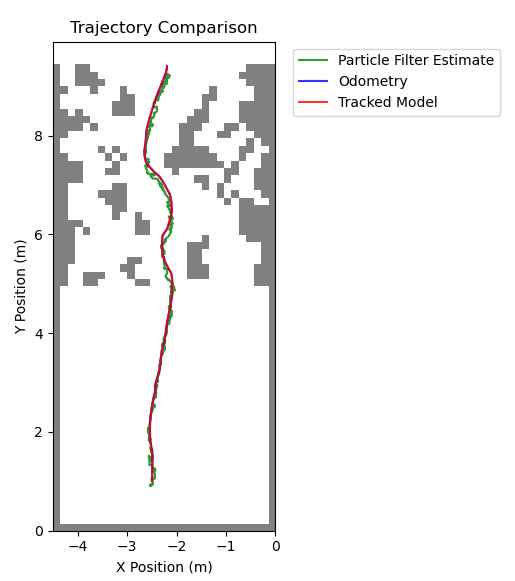
\includegraphics[width=1\linewidth]{combined_traj_sim.png}
    \caption{Visualization of the robot trajectories in world 250 from the BARN dataset. The odometry reading and the tracked model overlap with each other.}
    \label{fig:sim_traj}
\end{figure}
When implemented, and deployed on a real-world robot, as depicted in Figure \ref{fig:real_traj}, and Table \ref{tab:errors} this advantage is lost. The IMU based odometry no longer out-performs the particle filter with the IMU based odometry having an average distance of 0.67m compared to the ground truth. Meanwhile the particle filter has an average distance 0.59m compared to the ground truth. From Figure \ref{fig:real_traj} the error of the particle filter is high when compared to the results found in simulation, about 0.3m of offset. The 0.3m offset arises from the robot’s velocity (1m/s) divided by the particle filter’s update rate (3Hz), yielding \(\sim\)0.33m per update cycle. This latency was not subtracted from reported errors.
\begin{figure}[H]
    \centering
    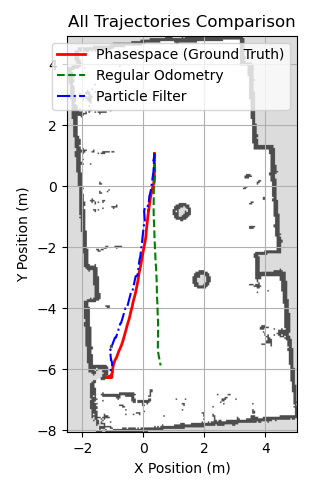
\includegraphics[width=1\linewidth]{combined_trajectories_robot.png}
    \caption{Both robot particle filter estimate as well as odometry readings, plotted with the tracked model position using the Phasespace system.}
    \label{fig:real_traj}
\end{figure}
\begin{table}
\centering
\caption{Localization Error Comparison}
\label{tab:errors}
\begin{tabular}{lcc}
\toprule
\textbf{Configuration} & \textbf{Simulation (m)} & \textbf{Real-World (m)} \\
\midrule
IMU-only & 0.0003 & 0.67 \\
IMU+LiDAR & 0.22 & 0.59 \\
\bottomrule
\end{tabular}
\end{table}
Another aspect of the real-robot system that showcases the strength of sensor fusion is compounding sensor error. As depicted in \ref{fig:error_ot}, while the error rate of the IMU based odometry continues to increase, the particle filter's error rate stays stable. This means that if you plan to deploy robots for a long period, sensor fusion is a good way to mitigate this accumulating error.
\begin{figure}
    \centering
    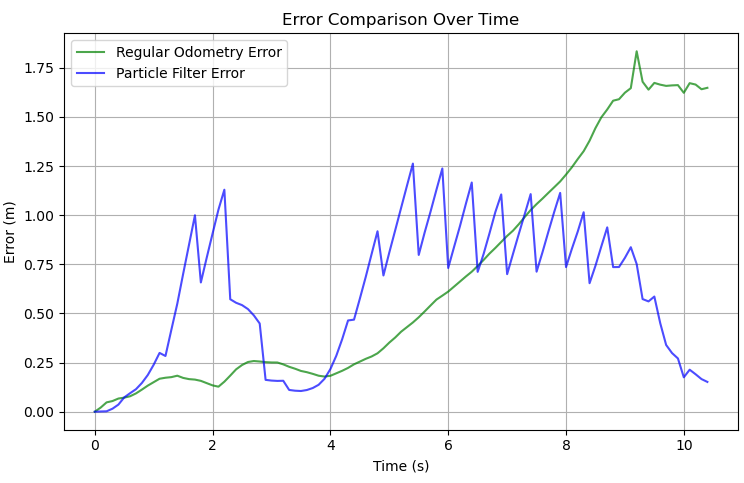
\includegraphics[width=1\linewidth]{error_plotted.png}
    \caption{The average error of each localization method plotted against time. It can be observed that the IMU based localization has accumulating error, while the particle filter based localization remains stable over time.}
    \label{fig:error_ot}
\end{figure}
\section{Discussion}
\subsection{Limitations}
In this experiment only two sensor configurations were tested. Future works should use more sensor configurations, such as depth-cameras, GPS, and/or other sensors that can be fitted on a robot. The particle filter’s 3Hz update rate introduced a latency-derived offset of \(\sim\)0.33m (1m/s / 3Hz). While this explains part of the error, it underscores the need for faster hardware or algorithmic optimizations like GPU acceleration. Using a stronger computer, or leveraging GPU acceleration could help mitigate this error.

\section{Conclusion}
In this work, a particle‐filter–based localization system that fuses IMU and LiDAR measurements was implemented and evaluated on the F1TENTH robotic platform.  In simulation, our LiDAR–IMU fusion achieved an average position error of 0.22m (versus 0.0003m for the idealized IMU‐only case), and on the real robot reduced mean localization error from 0.67m to 0.59m—a 11\% improvement in noisy environments.  Our particle filter maintained stable, bounded error over extended runs (see Fig.~\ref{fig:error_ot}).

These results demonstrate that even a minimal sensor suite of IMU and LiDAR can significantly mitigate odometric drift in both idealized and practical settings.  However, our approach incurs scan‐processing latency that was not subtracted from the error metrics, and performance can still degrade under heavy dynamic obstacles or poor LiDAR returns.  Moreover, parameter tuning for the process and measurement covariances remains manual and environment‐specific.

Future work will explore adaptive noise estimation to reduce manual calibration, integration of vision‐based features for richer landmark constraints, and a closed‐loop control evaluation to quantify end‐to‐end path‐tracking gains.  We also plan to open‐source our filter implementation and the synchronized sensor dataset to facilitate reproducibility and further research in low‐cost sensor fusion for autonomous robotics.

\section{Code and Acknowledgments}
This project was supported by the University of Minnesota's Office of
Undergraduate Research. All code used in this project can be found in this GitHub repository, \url{https://github.com/tubbleWeek/WCHAS_UROP_2025}. 

\section{Hyper parameters}
For both the simulation and real-world experiments, these hyper parameters were kept constant.
\begin{enumerate}
    \item Number of Particles: 100
    \item Lidar Sensor Model:
    \begin{itemize}
        \item z-hit: 0.85
        \item z-rand: 0.15
        \item sigma-hit: 0.1
    \end{itemize}
    \item Motion Model:
    \begin{itemize}
        \item alpha1: 0.1
        \item alpha2: 0.1
        \item alpha3: 0.1
        \item alpha4: 0.1
    \end{itemize}
\end{enumerate}
alpha1 and alpha 3 are the expected translational noise in the robot's IMU readings, while alpha2 and alpha4 are the expected rotational noise in the robot's IMU readings.
% --- Bibliography and Appendix Placeholders ---
\bibliographystyle{acl_natbib} % Or another appropriate style
\bibliography{bibliography} % Add your .bib file name here if you have one


% \appendix
% \section{Appendix Title}
% \label{sec:appendix}
% Appendix content goes here.

\end{document}